%%% 第二章
\chapter{吸收填料塔工艺参数计算}

按上述基本逻辑,进行吸收填料塔工艺参数的设计\cite{Design-of-Packed-Absorption-Column},具体步骤如下。

%%% ===============================================
\section{基础物性数据}

\subsection{气相物性数据}

对于气相,重要的物性包括混合气体的平均摩尔质量、混合气体的平均密度和混合气体的黏度。而混合气体的黏度由于\ce{SO2}含量较低,混合气体黏度可以近似取为空气的黏度。已知\ce{SO2}的摩尔质量$M_{\ce{SO2}}$为$64.06 \, g/mol$,空气的摩尔质量$M_{Air}$为$28.95 \, g/mol$,理想气体常数$R=8.314 \, m^3 \cdot kPa/(kmol \cdot K)$,则所需数据按理想气体状态方程计算如下:

混合气体的平均摩尔质量:
\begin{equation}
	\overline{M_{V}} = 0.060 \times 64.06 + (1-0.060) \times 28.95 = 31.0566 \, g/mol
\end{equation}

混合气体的平均密度为:
\begin{equation}
	\rho_{V}=\frac{PM_{V}}{RT}=\frac{120\times31.0566}{8.314\times(273.15+20)}=1.4291 \, kg/m^3
\end{equation}

混合气体黏度可近似取为空气黏度。查化工原理上册教材附录338页,得20°C时空气的黏度:
\begin{equation}
	\mu_{V}	= \mu_{Air}=1.81\times10^{-5} \, Pa \cdot s = 0.060 \, kg/(m \cdot h)
\end{equation} 

查化工原理课程设计得20°C时\ce{SO2}在空气中的扩散系数:
\begin{equation}
	D_{V}=0.108 \, cm^2/s = 0.039 \, m^2/h
\end{equation}

\subsection{液相物性数据}

对于低浓度吸收过程,溶液的物性数据可近似取水的物性数据。重要的液相物性包括密度、黏度、表面张力和\ce{SO2}在水中的扩散系数。由化工原理实验教材127页水的重要物理性质表得20°C时水的有关物性数据如下:

水的密度:
\begin{equation}
	\rho_{L} = 998.2 \, kg/m^3
\end{equation}

水的黏度:
\begin{equation}
	\mu_{L} = 1.005 \, mPa \cdot s = 0.001005 Pa \cdot s = 3.618 \, kg/(m \cdot h)
\end{equation}

水的表面张力:
\begin{equation}
	\sigma_{L} = 7.28 \times 10^{-2} = 0.0728\, N/m
\end{equation}

\ce{SO2}在水中的扩散系数:
\begin{equation}
	D_{L} = 1.47 \times 10^{-9} \, m^2/s = 5.292 \times 10^{-6} \, m^2/h
\end{equation}

\subsection{气液相平衡数据}

在吸收塔设计中,气液相平衡数据是确定传质驱动力的关键。对于\ce{SO2}在水中的溶解,我们需要考虑亨利系数、相平衡常数和溶解度系数。查教材82页表2-1得,常压下20°C时\ce{SO2}在水中的相关数据如下:

亨利系数:
\begin{equation}
	E = 0.355 \times 10^{4} = 3.55 \times 10^{3} \, kPa
\end{equation}

相平衡常数:
\begin{equation}
	m = \frac{E}{P} = 29.5833
\end{equation}

溶解度系数:
\begin{equation}
	H = \frac{\rho_{L}}{EM_{\ce{SO2}}} = 0.0156039 \, kmol/(kPa \cdot m^3)
\end{equation}
其中,$P$为系统压力,$\rho_{L}$为液相密度,$M_{\ce{SO2}}$为\ce{SO2}的摩尔质量。



%%% ===============================================
\section{物料衡算}

根据设计要求得知,进口气体的体积流量 $V'=1000 \, m³/h$,二氧化硫的摩尔分数为 $y_1=0.060$,二氧化硫吸收率 $η=98\%$。

进塔气相摩尔比:
\begin{equation}
	Y_1 = \frac{y_1}{1-y_1} = 0.0638298
\end{equation}

出塔气相摩尔比:
\begin{equation}
	Y_2 = Y_1(1-η) = 0.0012766
\end{equation}

进塔惰性气相流量:
\begin{equation}
	V = \frac{V'}{22.4} \times (1-y_1) \times \frac{273}{273+20} = 39.0998 \: kmol/h
\end{equation}

该吸收过程属于低浓度吸收,平衡关系为直线,因此最小液气比为:
\begin{equation}
	\left(\frac{L}{V}\right)_{min} = \frac{Y_1 - Y_2}{Y_1/m - X_2} = 28.9917
\end{equation}
式中:$X_2=0$,$L$ 为液相流量,$V$ 为气相流量。

一般情况下,吸收剂用量为吸收剂最小用量的 $1.1 \sim 2.0$ 倍,这里取操作液气比为 $1.4$ 倍最小液气比。
\begin{equation}
	\frac{L}{V} = 1.4 \left(\frac{L}{V}\right)_{min} = 40.5883
\end{equation}

吸收剂用量:
\begin{equation}
	L = 40.5883 \times 39.0998 = 1587 \: kmol/h
\end{equation}

物料衡算:
\begin{equation}
	V(Y_1-Y_2) = L(X_1-X_2)
\end{equation}
得 $X_1 = 0.00154116$



%%% ===============================================
\section{填料塔工艺尺寸计算}

相关塔径计算相关逻辑流程图如下:
\begin{figure}[h]
	\centering
	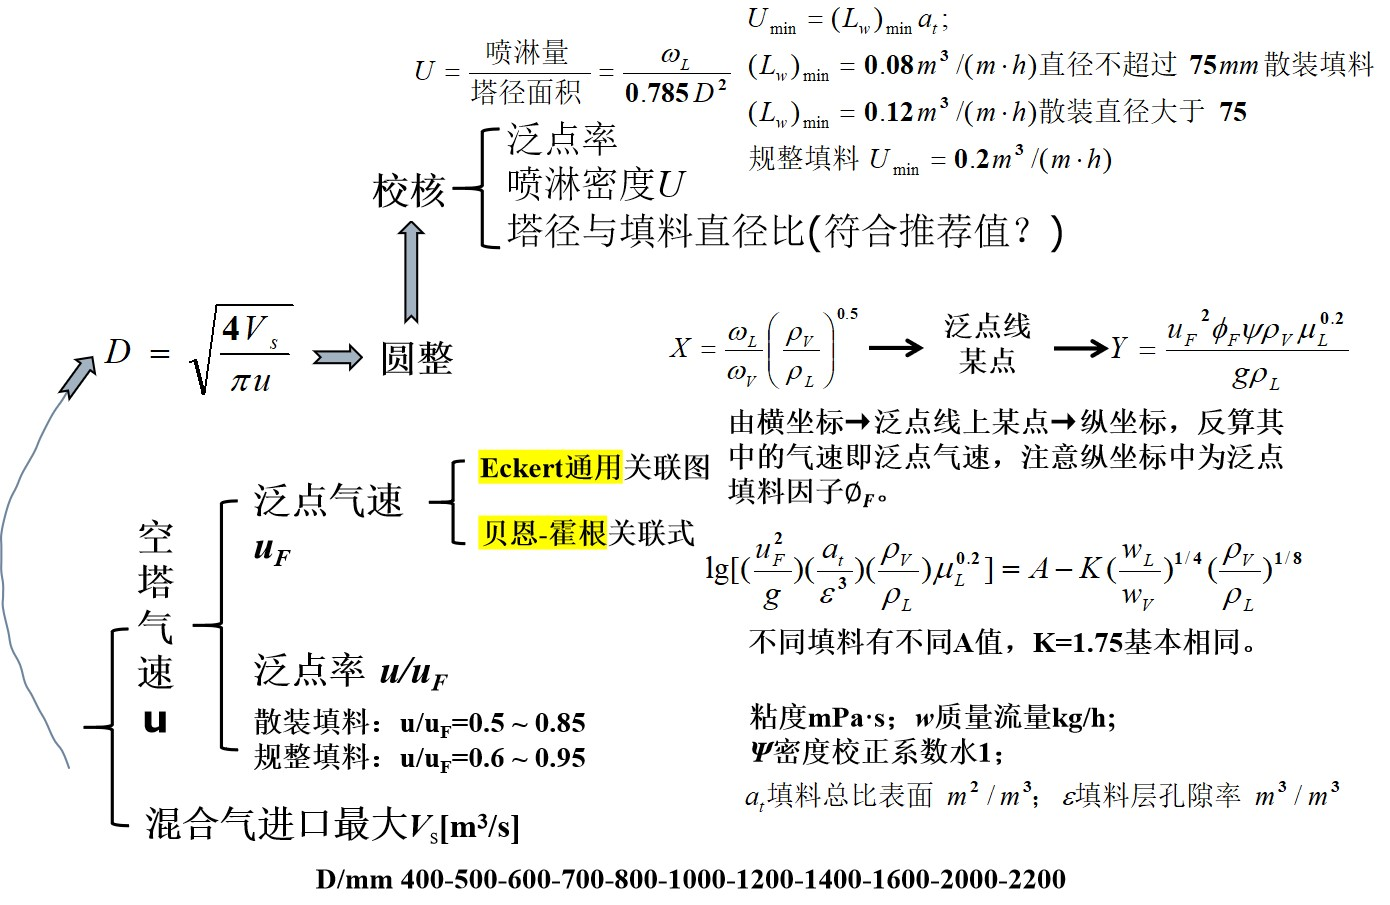
\includegraphics[width=0.8\textwidth]{塔径设计相关逻辑.jpg}
	\captionsetup{skip=2pt} % 内部定义的captionsetup,设置描述与图的间距
	\caption{泛点气速-塔径相关逻辑示意图}
\end{figure}

\subsection{填料塔塔径的计算}

采用 Eckert 通用关联图计算泛点气速。液相质量流量可近似按纯水流量计算,即液相质量流量为:
\begin{equation}
	W_{L} = 1587 \times 18.02 = 28597.7 \, kg/h
\end{equation}

气相质量流量为:
\begin{equation}
	W_{V} = 1000 \times 1.4291 = 1529.1 \, kg/h
\end{equation}

Eckert 通用关联图的横纵坐标值分别为:
\begin{equation}
	X_{Eckert} = \frac{W_{L}}{W_{V}} \left( \frac{\rho_{V}}{\rho_{L}} \right)^{0.5} = 0.731989
\end{equation}

查 Eckert 通用关联图得:
\begin{equation}
	Y_{Eckert} = \frac{u_F^2 \phi \varphi \rho_{V}}{g \rho_{L} \mu_{L}^{0.2}} = 0.034
\end{equation}
式中:$u_F$ 为泛点气速,m/s;$\rho_{V}$ 为气相密度,kg/m³;$\rho_{L}$ 为液相密度,kg/m³;$\mu_{L}$ 为液体黏度,mPa·s;$\phi$ 为实验填料因子,$g$ 为重力加速度,9.81 m/s²;$\varphi$ 为水的密度与液体密度之比,此处为$1$。

由化工原理课程设计教材 148 页表 6-4 得 $\phi = 184 \, m^{-1}$,则:

\begin{equation}
	u_F = \sqrt{\frac{Y_{Eckert} g \rho_{L}}{\phi \varphi \rho_{V} \mu_{L}^{0.2}}} = \sqrt{\frac{0.034 g \rho_{L}}{\phi \varphi \rho_{V} \mu_{L}^{0.2}}} = 0.9 28879 \, m/s
\end{equation}

取 $u = 0.7 u_F = 0.440215 \, m/s$,有:

\begin{equation}
	D = \sqrt{\frac{4V_{s}}{\pi u}} = \sqrt{\frac{4 \times 1000/3900}{3.14 \times 0.440215}} = 0.896337 \, m = 896.337 \, mm
\end{equation}
圆整塔径,取$D=0.9 m$,也即$D=900mm$。

\subsection{填料塔塔径的校核}

\textbf{泛点率校核}:
泛点率是塔内实际操作气速与泛点气速的比值,一般要求在 50\% $\sim$ 80\%之间。
\begin{equation}
	u =(1000/3900)/(\frac{\pi}{4} \times 0.9 ^2)= 0.436639 m/s
\end{equation}
\begin{equation}
	u/u_{F} = 0.436639 / 0.9 28879 = 0.694313 \text{ (在允许范围 0.50-0.85 之内)}
\end{equation}

\textbf{填料规格校核}:

当塔径与填料外径之比(即径比)过小时,塔的性能会变得不稳定。因为径比过小时,靠近塔壁的填料层的空隙率会增大且不均匀,塔的通过能力虽然会有所提升,但由于气流短路,塔的效率反而会下降。所以需要对填料规格进行校核,以下是常用填料的径比下限。

\begin{table}[h]
	\centering
	\caption{填料种类及其推荐值} % 添加表格标题
	\begin{tabularx}{\textwidth}{|X|X|} % 控制表格宽度为文本宽度
		\hline 
		\textbf{填料种类} & \textbf{$D/d$ 推荐值} \\
		\hline 
		拉西环 & $D/d \geq 20 \sim 30$ \\
		\hline 
		鞍环 & $D/d \geq 15$ \\
		\hline 
		鲍尔环 & $D/d \geq 10 \sim 15$ \\
		\hline 
		阶梯环 & $D/d > 8$ \\ % 修改了这里的符号
		\hline 
		环矩鞍 & $D/d > 8$ \\
		\hline
	\end{tabularx}
\end{table}
进行校核有:
\begin{equation}
	D/ d = 900/ 38 = 23.6842 > 10
\end{equation}

\textbf{液体喷淋密度校核}:
最小润湿速率是指塔的截面上,单位长度的填料周边的最小液体流体体积。直径不超过 75 mm 的散装填料,最小润湿速率为:
\begin{equation}
	(L_{W})_{min}=0.08m^{3}/(m \cdot h)
\end{equation}

由化工原理教材 325 页的聚丙烯鲍尔环特性数据表得
\begin{equation}
	a_{t}=175 \, m^2/m^3
\end{equation}
\begin{equation}
	U_{\min}=(L_{W})_{\min}a_{t}=14m^{3}/(m^{2}\cdot h)
\end{equation}
\begin{equation}
	U=\frac{28597.7/998.2}{\frac{\pi}{4}\times0.9 ^2}=45.0338 m^3/(m^2\cdot h)>U_{min}
\end{equation}
故满足最小喷淋密度的要求。经以上校核可知,填料塔直径 $D=900 mm$ 合理。

\subsection{传质单元数的计算}

脱析因数 \( S \) 计算如下:
\begin{equation}
	S = \frac{mV}{L} = \frac{29.5833}{40.5883} = 0.728863
\end{equation}

气相总传质单元数 \( N_{OG} \) 的计算为:
\begin{align}
	N_{OG}
	&= \frac{1}{1-S} \ln \left[\left(1-S\right)\frac{Y_1 - Y_2^{*}}{Y_2 - Y_2^{*}} + S\right] \\
	&= \frac{1}{1-0.728863} \ln \left[\left(1-0.728863\right)\frac{0.0582-0}{0.002328-0}+0.728863\right] \notag \\
	&= 9.80781  \notag
\end{align}

\subsection{膜吸收系数的计算}

\begin{figure}[h]
	\centering
	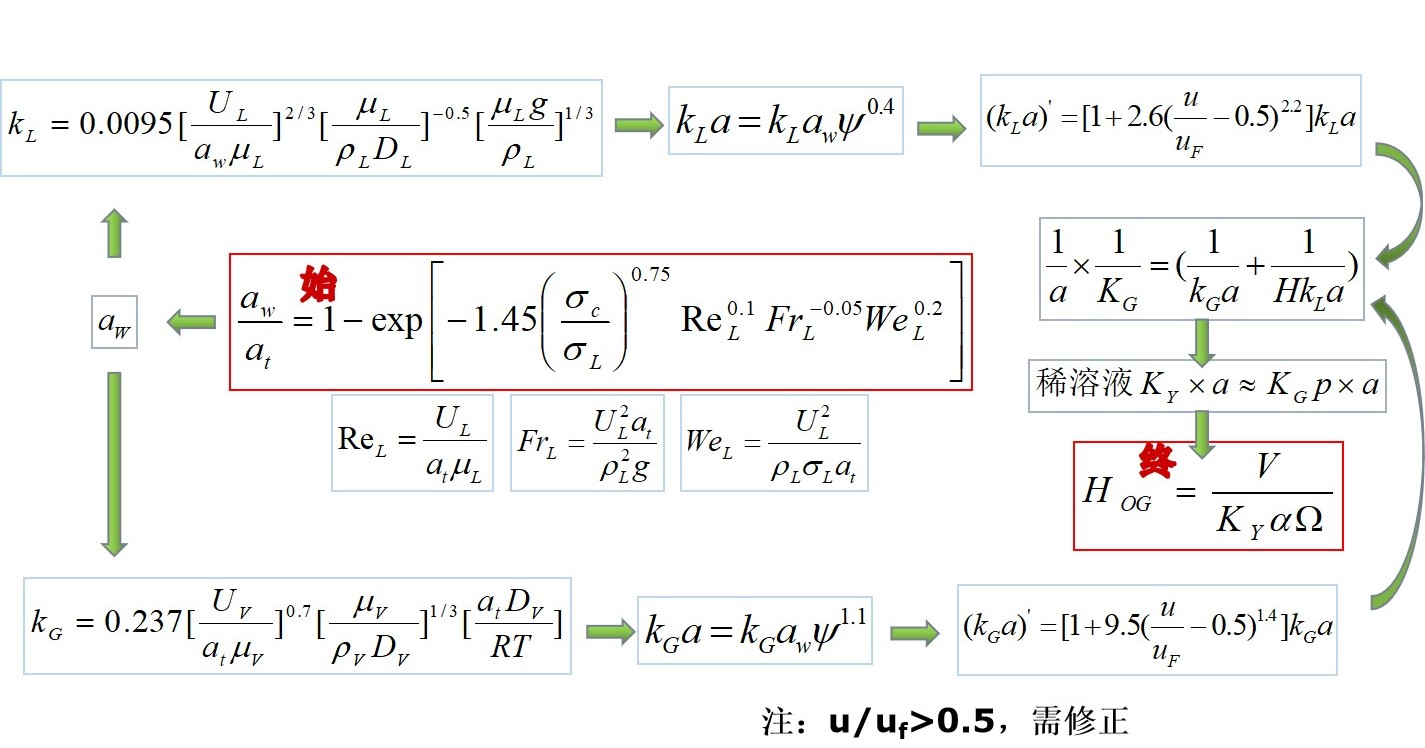
\includegraphics[width=0.8\textwidth]{传质单元高度.jpg}
	\caption{由膜吸收系数至传质单元高度的流程示意图}
\end{figure}

气相总传质单元高度采用修正的Onda关联式:
\begin{equation}
	\frac{a_{w}}{a_{t}} = 1-e^{-1.45\left(\frac{\sigma_c}{\sigma_w}\right)^{0.75}\left(\frac{U_{L}}{a_{t}\mu_{L}}\right)^{0.1}\left(\frac{U_{L}\mu_{L}}{\rho_{L}g}\right)^{-0.05}\left(\frac{U_{L}^2}{\rho_{L}\sigma_L a_{t}}\right)^{-0.2}}
\end{equation}

由化工原理课程设计教材中175页表6-6得$\sigma_{c} = 427680kg/h^{2}$

液体质量通量:
\begin{equation}
	U_{L} = \frac{28597.7}{\frac{\pi}{4} \times 0.9 ^2} = 44952.7 kg/(m^2·h)
\end{equation}

代入Onda关联式:
\begin{equation}
	\frac{a_{w}}{a_{t}} = 0.443873
\end{equation}

所以:
\begin{equation}
	a_{w} = 0.443873 \times 175 = 77.6778 \, m^2/m^3
\end{equation}

气体质量通量:
\begin{equation}
	U_{V} = \frac{1529.1}{\frac{\pi}{4} \times 0.9 ^2} = 2403.59 kg/(m^2·h)
\end{equation}

计算气侧吸收系数:
\begin{align}
	k_{G}
	&= 0.237\Bigg(\frac{U_{V}}{a_{t}\mu_{V}}\Bigg)^{0.7}\Bigg(\frac{\mu_{V}}{\rho_{V}D_{V}}\Bigg)^{1/3}\Bigg(\frac{a_{t}D_{V}}{RT}\Bigg) \\
	&=
	0.0288785 \, kmol/(m^2·h·kPa) \notag
\end{align}

计算液膜吸收系数:
\begin{align}
	k_{L}
	&= 0.0095\biggl(\frac{U_{L}}{a_{w}\mu_{L}}\biggr)^{2/3}\biggl(\frac{\mu_{L}}{\rho_{L}D_{L}}\biggr)^{-1/2}\biggl(\frac{\mu_{L}g}{\rho_{L}}\biggr)^{1/3} \\
	&=
	0.826184 \, m/h \notag
\end{align}

\subsection{总传质系数的计算}

\textbf{体积吸收系数}:

由化工原理课程设计教材175页表6-7得参数 $\psi = 1.45$,计算 $k_Ga$ 和 $k_La$ 如下:
\begin{align}
	k_{G}a
	&= k_{G}a_{W} \psi^{1.1} \\
	&= 0.0288785 \times 91.0681 \times 1.45^{1.1} \notag \\
	&= 3.3758 \, kmol/(m^3 \cdot h \cdot kPa) \notag
\end{align}
\begin{align}
	k_{L}a
	&= k_{L}a_{W} \psi^{0.4} \\
	&= 0.826184 \times 91.0681 \times 1.45^{0.4} \notag \\
	&= 74.4596 \, kmol/(m^3 \cdot h \cdot kPa) \notag
\end{align}

\textbf{修正体积吸收系数}:

由于 $u/u_F = 0.694313 > 0.5$,使用化工原理课程设计教材152页修正公式(6-12)与(6-13)进行修正:
\begin{align}
	k_{G}^{\prime}a
	&= \left[1 + 9.5 \left(\frac{u}{u_{F}} - 0.5\right)^{1.4}\right] k_{G}a \\
	&= 6.61176 \, kmol/(m^3 \cdot h \cdot kPa) \notag
\end{align}
\begin{align}
	k_{L}^{\prime}a
	&= \left[1 + 2.6 \left(\frac{u}{u_{F}} - 0.5\right)^{2.2}\right] k_{L}a \\
	&= 79.727 \, kmol/(m^3 \cdot h \cdot kPa) \notag
\end{align}

\textbf{总体积传质系数}:
\begin{equation}
	K_{G}a = \frac{1}{\frac{1}{k_{G}^{\prime}a} + \frac{1}{H k_{L}^{\prime}a}} = 1.04705 \, kmol/(m^3 \cdot h \cdot kPa)
\end{equation}

\subsection{填料层高度的计算}

计算填料层高度 $H_{OG}$ 和总高度 $Z$:
\begin{equation}
	H_{OG} = \frac{V}{K_{G}a p_{总} \Omega} = 0.489162 \, m
\end{equation}
\begin{equation}
	Z = H_{OG} \cdot N_{OG} = 4.79761 \, m
\end{equation}
\begin{equation}
	Z^{\prime} = 1.25Z = 5.99701 \, m
\end{equation}
设计取填料层高度为 $Z^{\prime} = 4.1 \, m < h_{max} = 6 \, m$,故不进行分段。

\subsection{填料层压降的计算}
填料层压降直接影响到填料塔的能效和操作性能。压降的大小决定了塔内气体的流动状态,过高的压降会增加泵送能耗,降低塔的处理能力和操作灵活性。而过低的压降可能意味着填料层的传质效率不足,影响塔的分离效率。

在设计阶段,通过计算填料层压降,可以选择合适的填料类型和尺寸,以及确定塔的操作参数,确保塔在经济和技术上的可行性。在操作阶段,监控和调整填料层压降有助于维持塔内气液两相的理想流动状态,避免出现液泛等不稳定现象,从而保证塔的稳定运行和提高产品质量。 因此,填料层压降的计算是填料吸收塔设计和优化中的一个基本步骤,对于实现高效、节能和安全的化工生产具有重要意义。

\begin{figure}[h]
	\centering
	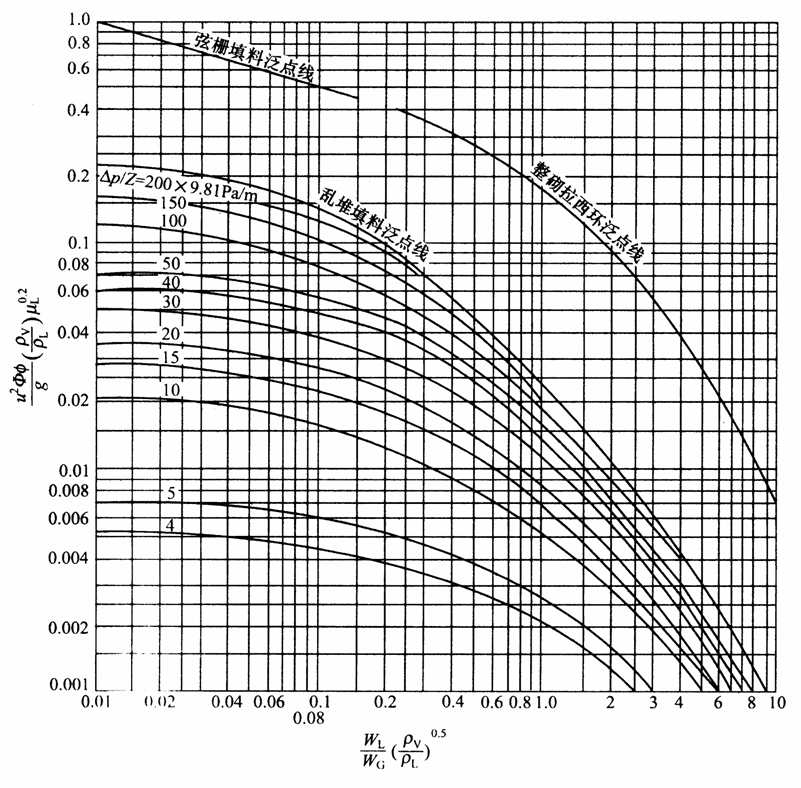
\includegraphics[width=0.6\textwidth]{Eckert关联图.png}
	\caption{Eckert通用关联图}
\end{figure}

采用埃克特通用关联图计算填料层压降,Eckert 通用关联图的横坐标值为:
\begin{equation}
	X_{Eckert} = \frac{W_{L}}{W_{V}} \left( \frac{\rho_{V}}{\rho_{L}} \right)^{0.5} = 0.731989
\end{equation}

查化工原理课程设计 154 页表 6-11$^{[3]}$可得$\phi_{p}=232m^{-1}$,则
纵坐标为:
\begin{equation}
	Y_{Eckert} = \frac{u_F^2 \phi_{p} \varphi \rho_{V}}{g \rho_{L} \mu_{L}^{0.2}} = 0.00893255
\end{equation}
式中:$u_F$ 为泛点气速,m/s;$\rho_{V}$ 为气相密度,kg/m³;$\rho_{L}$ 为液相密度,kg/m³;$\mu_{L}$ 为液体黏度,mPa·s;$\phi_{p}$ 为填料层压降的实验填料因子,$g$ 为重力加速度,9.81 m/s²;$\varphi$ 为水的密度与液体密度之比,此处为$1$。

查化工原理课程设计 148 页图 6-2,得单位填料层压降:
\begin{equation}
	\Delta p/Z = 9 \times 9.81 = 88.29 \, Pa/m
\end{equation}

则填料层压降:
\begin{equation}
	\Delta p=88.29\times5.7 \, Pa = 503.253 \, Pa
\end{equation}

\subsection{塔附属高度的计算}
塔的附属高度包括上部空间、液体分布器空间和底部空间。根据设计,塔的上部空间取1.0米,底部空间取1.1米,液体分布器高度为0.2米,因此塔的附属高度为:

\begin{equation}
	H_{\text{附属}} = 1.0 + 1.1 + 0.2 = 2.3 \, m
\end{equation}



%%% ===============================================
\section{吸收塔工艺尺寸总结}
吸收塔工艺计算的目的是确保设备能够在实际操作中高效、稳定地进行传质操作,并满足设计要求。通过严密的气液传质模型和物料衡算,我们能够设计出适合特定工艺条件的吸收塔。

首先,在物性数据的获取与应用中,通过对气液相物理性质如密度、黏度、扩散系数等的准确估算,保证了后续计算的可靠性。特别是亨利系数等气液相平衡数据的获取,为传质驱动力的计算提供了坚实的基础。

在物料衡算中,基于已知的气体流量、二氧化硫的浓度及吸收率,计算出进出塔的气相摩尔比、惰性气体流量及最小液气比,并确定了实际操作中的液气比。通过这些数据,可以进一步推导出吸收剂的用量,确保吸收操作能够实现高效的二氧化硫去除。

随后,在填料塔的尺寸设计中,利用Eckert通用关联图和相关实验参数,计算出泛点气速、塔径及填料层高度,并进行了校核。通过对泛点率、填料规格及液体喷淋密度的核查,确保塔的设计既能满足工艺需求,又不会出现气流短路或液泛等不良现象。此外,对填料层压降的计算也表明塔内流体流动阻力在合理范围内,保证了塔的能耗在可接受的范围。

在传质计算中,应用膜吸收系数、Onda关联式以及修正体积吸收系数,确保了传质效率的准确估计。通过计算气侧和液侧的传质单元数及传质单元高度,得出合适的填料层高度,保证气液传质能够在塔内有效进行。

最后,通过附属高度的设计,包括塔的上部空间、液体分布器及底部空间的合理布置,确保塔的整体结构稳定性和操作便利性。在附属设备的设计中,液体分布器和再分布器的合理配置,能够有效改善塔内流体的分布,减少局部液体聚集或气流短路的情况,从而进一步提高塔的效率。

总而言之,吸收塔的工艺计算不仅包括物料衡算、传质单元和填料层高度等核心内容,还涉及到结构设计、流体力学参数和操作稳定性的校核。通过这一系列精确的计算与校核,吸收塔的设计可以确保其在实际工业操作中具有高效的传质性能和良好的操作稳定性,从而实现高效的二氧化硫吸收和废气处理目标。

\clearpage

\begin{longtable}{
		@{} p{0.30\textwidth} p{0.20\textwidth} 
		p{0.20\textwidth} p{0.25\textwidth} @{}
		}
	\caption{参数汇总表} \\
	\toprule
	描述信息 & 参数符号 & 参数值 & 单位 \\
	\midrule
	\endfirsthead
	
	\toprule
	描述信息 & 参数符号 & 参数值 & 单位 \\
	\midrule
	\endhead
	
	\midrule
	\multicolumn{4}{r}{\textit{——接下页}} \\
	\endfoot
	
	\bottomrule
	\endlastfoot
	
	摩尔质量 & $M_V$ & $31.0566$ & g/mol \\
	气体密度 & $\rho_V$ & $1.4291$ & kg/m³ \\
	气体扩散系数 & $D_V$ & $1.08 \times 10^{-5}$ & m²/s \\
	气体粘度 & $\mu_V$ & $1.81 \times 10^{-5}$ & Pa·s \\
	亨利常数 & $E$ & $3550$ & kPa \\
	气体分子质量比 & $m$ & $29.5833$ & - \\
	液体密度 & $\rho_L$ & $998.2$ & kg/m³ \\
	液体粘度 & $\mu_L$ & $1.005 \times 10^{-3}$ & Pa·s \\
	表面张力 & $\sigma_L$ & $0.0728$ & N/m \\
	液体扩散系数 & $D_L$ & $1.47 \times 10^{-9}$ & m²/s \\
	溶解度系数 & $H$ & $0.0156039$ & kmol/(kPa·m³) \\
	进料气体组分 & $Y_1$ & $0.0638298$ & - \\
	出料气体组分 & $Y_2$ & $0.0012766$ & - \\
	气体流量 & $V$ & $39.0998$ & kmol/h \\
	液气比 & $\left(\frac{L}{V}\right)_{min}$ & $28.9917$ & - \\
	最小液气比 & $\left(\frac{L}{V}\right)_{min\_ratio}$ & $1.4$ & - \\
	实际液气比 & $\frac{L}{V}$ & $40.5883$ & - \\
	液体流量 & $L$ & $1587$ & kmol/h \\
	进料液体组分 & $X_1$ & $0.00154116$ & - \\
	液体质量流量 & $W_L$ & $28597.7$ & kg/h \\
	气体质量流量 & $W_V$ & $1529.1$ & kg/h \\
	泛点气速Eckert坐标X值 & $X_{Eckert, \phi_F}$ & $0.731989$ & - \\
	泛点气速Eckert坐标Y值 & $Y_{Eckert, \phi_F}$ & $0.034$ & - \\
	泛点气速 & $u_F$ & $0.9 28879$ & m/s \\
	设计气速 & $u_{design}$ & $0.440215$ & m/s \\
	未圆整塔径 & $D$ & $0.896337$ & m \\
	圆整后塔径 & $D_{rounded}$ & $0.9$ & - \\
	实际操作气速 & $u_{actual}$ & $0.436639$ & m/s \\
	泛点率 & $flooding \, ratio$ & $0.9 94313$ & - \\
	圆整后塔径与填料直径比 & $\frac{D_rounded}{d}$ & $23.6842$ & - \\
	最小喷淋密度 & $U_{min}$ & $14$ & m³/(m²·h) \\
	实际喷淋密度 & $U$ & $45.0338$ & m³/(m²·h) \\
	脱吸因数 & $S$ & $0.728863$ & m² \\
	气相总传质单元数 & $N_{OG}$ & $9.80781$ & - \\
	液相质量通量 & $U_L$ & $44952.7$ & kg/(m²·h) \\
	有效比表面积比 & $\frac{a_w}{a_t}$ & $0.443873$ & - \\
	有效比表面积 & $a_w$ & $77.6778$ & m²/m³ \\
	气相质量通量 & $U_V$ & $2403.59$ & kg/(m²·h) \\
	气膜吸收系数 & $k_G$ & $0.0288785$ & kmol/(m²·h·kPa) \\
	液膜吸收系数 & $k_L$ & $0.826184$ & m/h \\
	气膜体积吸收系数 & $k_{G}a$ & $3.3758$ & kmol/(m²·h·kPa) \\
	液膜体积吸收系数 & $k_{L}a$ & $74.4596$ & m/h \\
	修正后的气膜体积吸收系数 & $k'_{G}a$ & $6.61176$ & kmol/(m²·h·kPa) \\
	修正后的液膜体积吸收系数 & $k'_{L}a$ & $79.727$ & m/h \\
	总传质系数 & $K_{G}a$ & $1.04705$ & kmol/(m²·h·kPa) \\
	填料层高度 & $H_{OG}$ & $0.489162$ & m \\
	总高度 & $Z$ & $4.79761$ & m \\
	设计高度 & $Z'$ & $5.99701$ & m \\
	填料层压降Eckert坐标X值 & $X_{Eckert, \phi_P}$ & $0.731989$ & - \\
	填料层压降Eckert坐标Y值 & $Y_{Eckert, \phi_P}$ & $0.00893255$ & - 
\end{longtable}